\documentclass[a4paper,9pt, twocolumn]{article}

\usepackage[utf8]{inputenc}
\usepackage[T1]{fontenc}
\usepackage{lmodern}
\usepackage{amsthm}
\usepackage{amsmath}
\usepackage{amssymb}
\usepackage{mathrsfs}
\usepackage{amsfonts}
\usepackage[top=1.5cm, bottom=2.2cm, left=2cm, right=2cm]{geometry}
\usepackage{fancyhdr}
\usepackage{graphicx}
\usepackage{multicol}
\usepackage{enumerate}
\usepackage{alltt}
\usepackage[svgnames]{xcolor}
\usepackage[francais]{babel}
\pagestyle{fancy}

\fancyhf{}
\renewcommand{\headrulewidth}{0pt}
\fancyfoot[C]{\tiny{Che Bedara - BDE Télécom ParisTech}}
\fancyfoot[RO]{\thepage}
\fancyfoot[LE]{\thepage}

\title{\vspace{-1.1cm} \textbf{Fiche de RES101} \vspace{-1.1cm}}
\date{}
\author{}

\begin{document}

\maketitle

\section*{Modèle OSI}

	\textbf{Def : le modèle OSI est né quand nous avons commencé à avoir une certaine expérience des communications entre ordinateurs. Son objectif est de normaliser les communications pour garantir un maximum d'évolutivité et d'interopérabilité entre les ordinateurs.}
	
	\begin{itemize}
		\item Le modèle OSI est un modèle en couches. Cela veut dire qu'il est découpé en plusieurs morceaux appelés couches.
		\begin{center}
		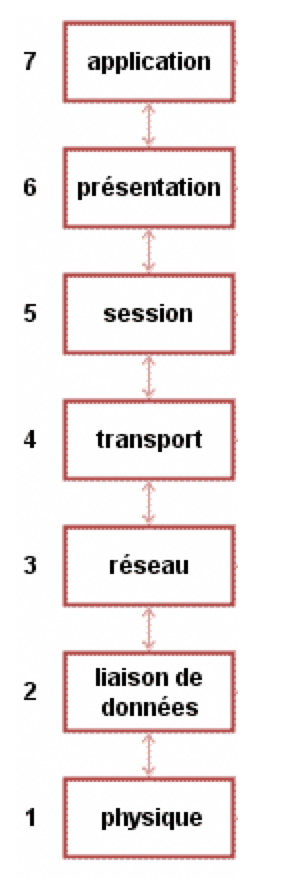
\includegraphics[scale=0.4]{couches.png}
		\end{center}
		\item Couche 1 : Physique $\Longrightarrow$ offrir un support de transmission pour la communication.
		\item Couche 2 : Liaison de données $\Longrightarrow$ connecter les machines entre elles sur un réseau local (+ détecter les erreurs et fiabiliser la connexion physique entre deux réseaux) $\Longrightarrow$ $Switch$
		\item Couche 3 : Réseau $\Longrightarrow$ interconnecter les réseaux entre eux, cad trouver un chemin pour envoyer des données d'un terminal à un autre à travers un réseau hétérogène et fragmenter les paquets $\Longrightarrow$ $Routeur$.
		\item Couche 4 : Transport $\Longrightarrow$ gérer les connexions applicatives et garantir la connexion.
		\item Couche 5 : Session (rarement implémentée).
		\item Couche 6 : Présentation $\Longrightarrow$ définit une syntaxe commune pour la représentation des données.
		\item Couche 7 : Application $\Longrightarrow$ source et destination des données à transporter.
	\end{itemize}

	\textbf{Deux règles pour les couches : }
	\begin{itemize}
		\item Chaque couche est indépendante (ex : Adressage IP (couche 3) peut être interchangeable (IPv4 $\Leftrightarrow$ IPv6) sans toucher aux autres couches).
		\item Chaque couche ne peut communiquer qu'avec une couche adjacente. (Envoi de données : de haut en bas $\neq$ Réception de données : de bas en haut).
	\end{itemize}

	\textbf{Principe de l'architecture des couches :}
	\begin{itemize}
		\item Les unités de données échangées : \textbf{SDU}.
		\item Les unités de données manipulées \textbf{PDU} (= SDU + \textbf{PCI} (champs spécifique au control du protocole)).
			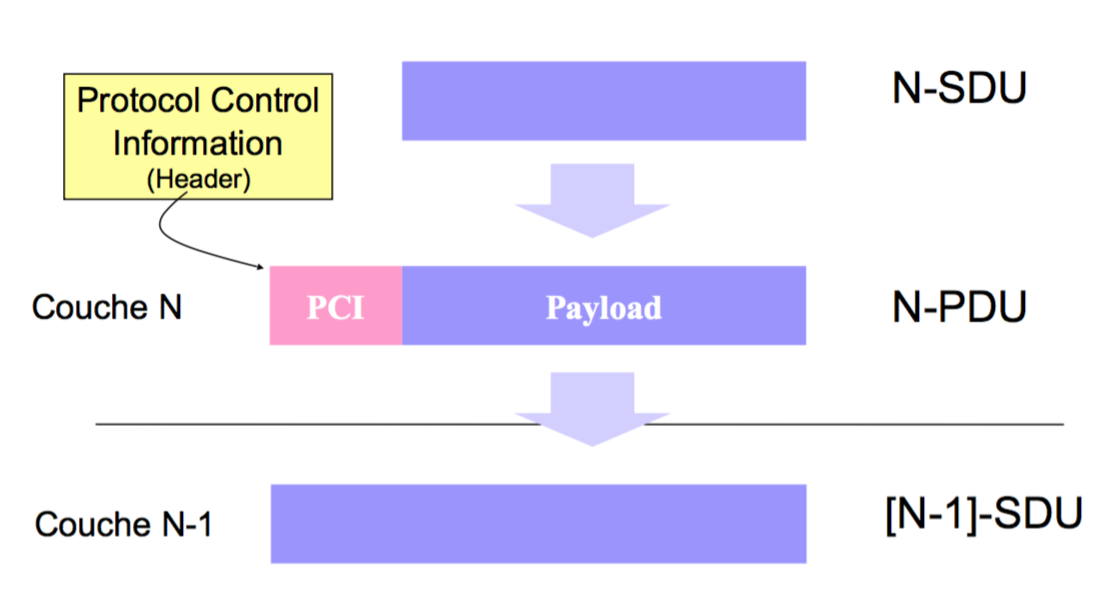
\includegraphics[scale=0.4]{PDU.png}
	\end{itemize}
	
	\textbf{TCP/IP vs OSI Model :}
	\begin{center}
		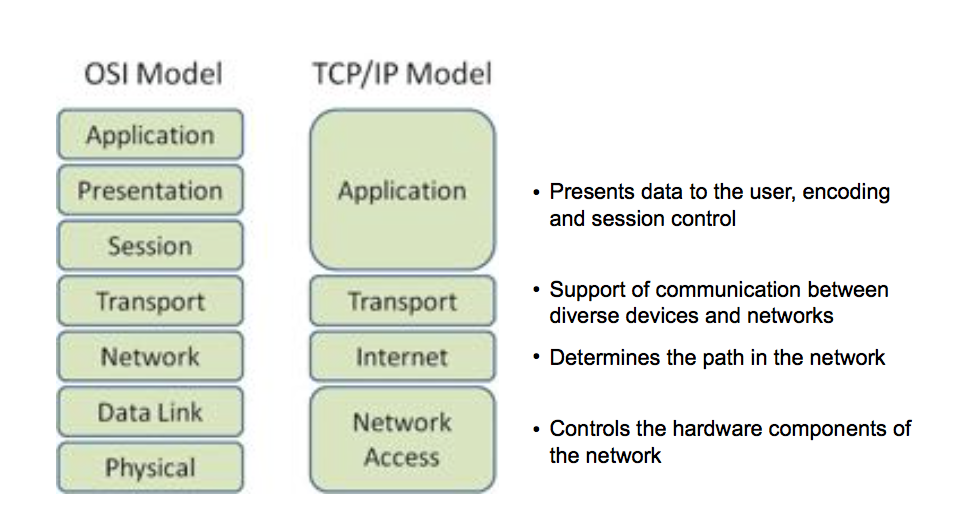
\includegraphics[scale=0.4]{TCP.png}
	\end{center}


\section*{Réseaux locaux (PHY/MAC)}

	Problématique de l'accès partagé : il peut être intéressant de partager un même support physique/logique entre plusieurs terminaux. 
	\begin{itemize}
		\item Il existe deux type de transmission : asynchrone (peut débuter à n'importe quel instant) et synchrone (on divise le temps en intervalles $T$ et la transmission ne peut débuter qu'en début de slot).
		\item Il est existe deux types de stratégies : déterministe (qui évite les collisions en partageant les bandes) et aléatoire qui ne peuvent pas éviter les collisions.
	\end{itemize}
	
	\textbf{Protocole ALOHA/ALOHA discrétisé}
	\begin{itemize}
		\item \textbf{Principe ALOHA:} N stations envoient des données à une station centrale, une station est autorisée à émettre dès qu'elle a un paquet à envoyer.
		\item Émission sur la fréquence $f_{1}$ dès qu'elle a un paquet.
		\item Risque de perte de paquet si collision ou bruit du canal trop élevé.
		\item Si au bout d'un aller retour l'utilisateur ne reçoit pas d'acquittement, il ré-emet son paquet au bout d'un délai aléatoire.
		\item \textbf{Principe ALOHA discrétisé: } le temps est divisé en intervalles de temps égaux. Une station spéciale est chargée d'émettre un signal permettant la synchronisation des stations.
		\item \textbf{Critère de performance :} Débit normalisé (proportion du temps pendant lequel le canal est utilisé), Délai, Stabilité, Équité entre les stations.
	\end{itemize}

	\textbf{CSMA/CSMA-CD : Protocoles à détection de porteuse} : les stations adapent leur comportement à l'activité du canal (si occupé, il ne faut pas émettre, et s'il est libre on transmet). Plusieurs types :
	\begin{itemize}
		\item CSMA 1-persistant : Lorsque le canal est libre, l'émission se fait avec une probabilité 1 $\longrightarrow$ proba de collision élevé si le trafic est important.
		\item CSMA non persistant : si canal occupé on introduit une attente aléatoire en plus $\longrightarrow$ probabilité de collision réduite.
		\item CSMA p-persistent : si le canal n'est pas occupé on émet avec une probabilité $p$ (plus le nombre de stations est important, plus faible doit être $p$ et donc plus important est le délai).
		\item CSMA-CD : on peut émettre et sonder le signal simultanément, lorsqu'une collision est détectée, la transmission en cours est interrompu + Choix de la période d'attente (Binary Exponential Backoff BEB) : Après $i$ collision on attend de façon aléatoire entre $0$ et $2^{i}-1$.
			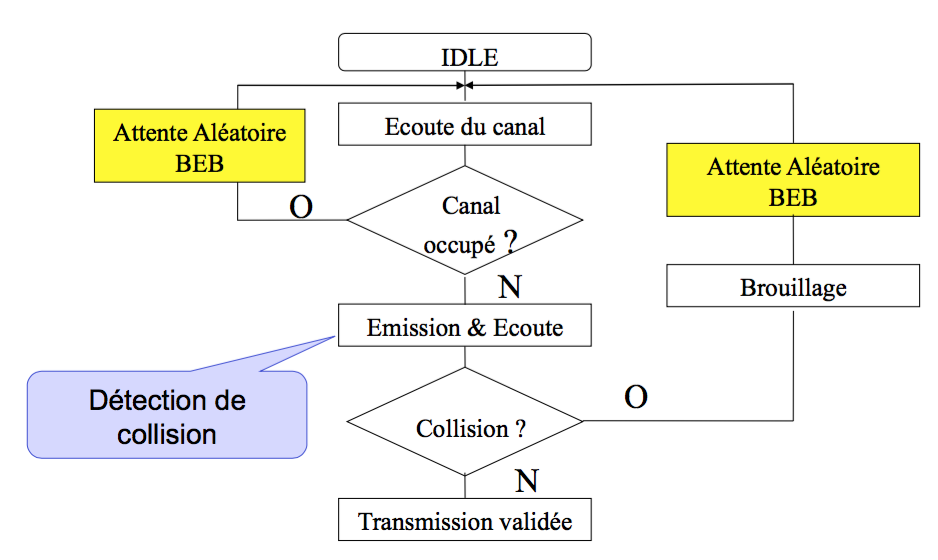
\includegraphics[scale=0.4]{CD.png}
		\item Paramètre $a = \tau /T$ le rapport période de vulnérabilité sur temps de propagation maximal. a est lié aux protocoles CSMA.
	\end{itemize}

	\textbf{Ethernet}
	\begin{itemize}
		\item Cable croisées à 8 fils (on utilise couramment 4 fils, deux à l'émission et deux à la transmission).
		\item Les câbles sont torsadés.
		\item La sortie est en général en RJ45.
			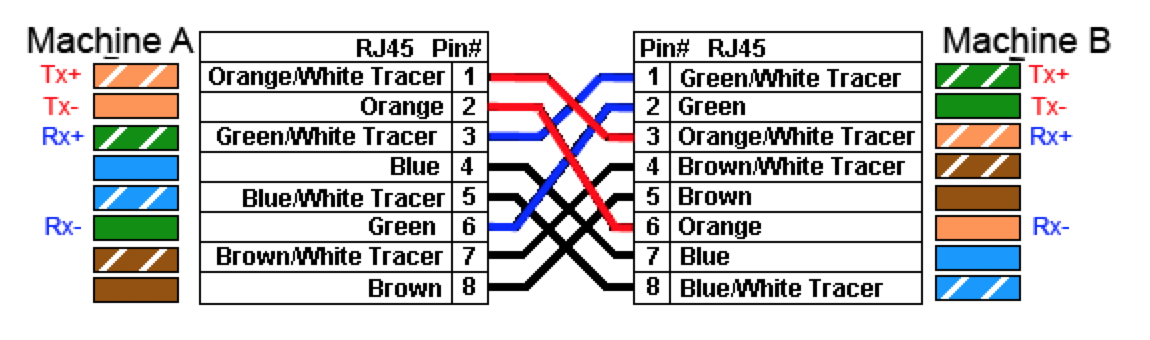
\includegraphics[scale=0.4]{RJ.png}
		\item Deux types de codage: codage en bande de base (narmol) et le codage de Manchester :
			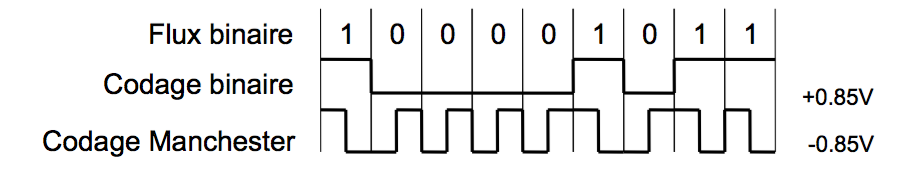
\includegraphics[scale=0.4]{code.png}
	\end{itemize}

	\textbf{Couches MAC}
	\begin{itemize}
		\item L'adresse MAC est universelle : une station s'attachant à un réseau est sur d'avoir une adresse unique. 
		\item Les 24 premiers bits sont assignés au constructeur par l'IEEE, les 24 derniers sont sont choisis par le constructeur de la carte
		\item l'adresse broadcast : \texttt{ff:ff:ff:ff:ff:ff}
		\item \textit{Contrôle de liaison logique (LLC)} : fiabilise une communication point à point (gestion des erreurs et controle de flux).
			Offre 3 types de service à une couche réseau $\longrightarrow$ mode sans connexion non-acquitté, mode orienté connexion, mode sans connexion avec acquittements.		
			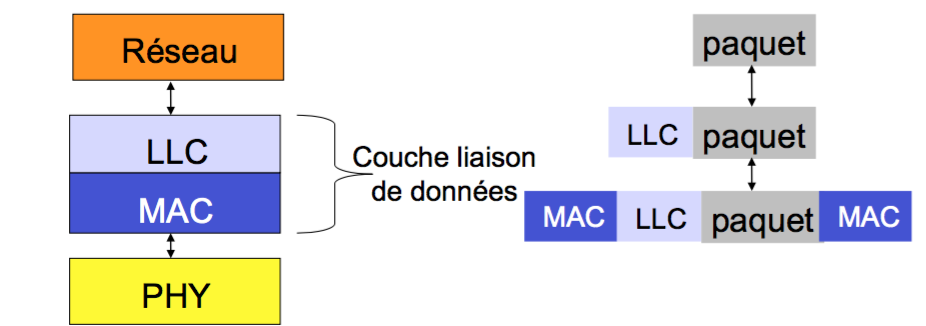
\includegraphics[scale=0.4]{LLC.png}
	\end{itemize}

	\textbf{Interconnexion des réseau locaux}
	\begin{itemize}
		\item Réparateur : Décode les données et transmet les données sur tous les segments auxquel il est attaché
		\item Concentrateur (Hub) : Topologie en étoile, connecte, des brins entre eux et diffuse sur toutes les branches de l'étoile.
		\item Les ponts (bridge) : Possède une adresse MAC et filtre les trames en  laissant passer les trames de broadcast.
		\item Spanning tree : Suppression des boucles dans des topologies de réseau contentant des chemins redondants (on ne garde qu'un seul chemin en bloquant l'accès aux autres).
			On construit un graphe non orienté et connecté et calcule le plus court chemin à la racine(fondé sur l'adresse MAC + priorité).
		\item Les commutateurs (switch) : 4 à 32 cartes comprenant chacune 8 ports.
		\item Les apports sur switch : plus de CSMA/CD, il n'y a plus de collision avec les switch, la carte réseau fonctionne en \textbf{full duplex}
	\end{itemize}


\section*{Réseau sans fil}

	\textbf{Classifications des réseaux sans fils :} 
	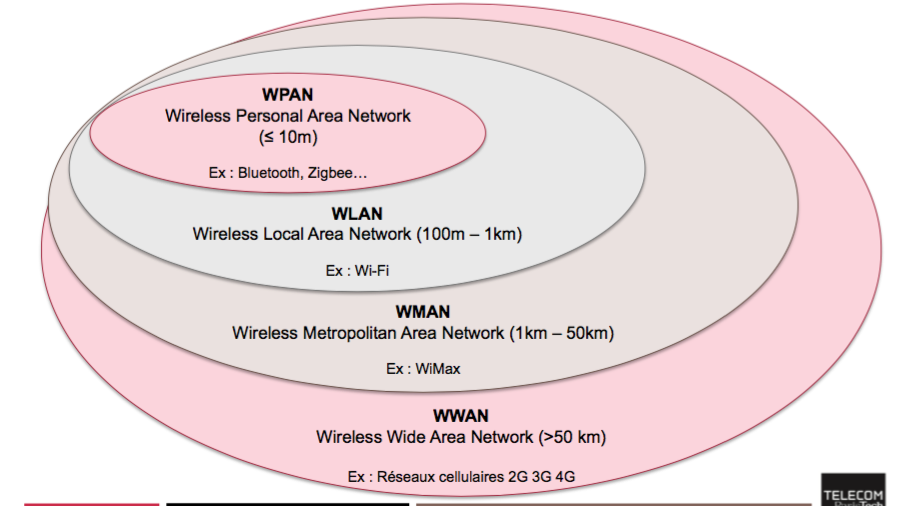
\includegraphics[scale=0.6]{res.png}
	
	\textbf{Propagation radio : } 
	$$P_{r} = P_{e} G_{e} G_{r} \left( \frac{K\lambda^{2}}{r^{\alpha}} \right) a_{\text{shadowing}} a_{\text{fading}}$$
	avec : 
	\begin{itemize}
		\item $\alpha$ : le coefficient d'atténuation (entre le vide et l'urbain)
		\item $a_{\text{shadowing}}$ : effet de masque (objet entre émetteur et récepteur)
		\item $a_{\text{fading}}$ : évanouissements rapide (variations raides du canal)
	\end{itemize}
	
	\textbf{Wi-Fi} - 2 bandes : 
	\begin{itemize}
		\item Entre 2.4 et 2.48 GHz (avec 13 canaux en Europe)
		\item Entre 5.15 et 5.35 GHz : pour les radars météo et les usages militaires.
		\item \textbf{CSMA/CA} : On écoute avant d'émettre.
			Quand le médium est libre, on attend un délai fixe avant d'émettre.
	\end{itemize}
	
	
\section*{Network (IP) Layer}

	Couche 3 : Interconnexion des réseaux (les couches 1 et 2 formaient les réseaux locaux, la couche 3 relie tout ces réseaux).
	
	\textbf{Adresse IP}
	\begin{itemize}
		\item Codée sur 32 bits (de \texttt{O.O.O.O} à \texttt{255.255.255.255})
		\item On ajoute une information supplémentaire à l'adresse IP qui est le masque de sous-réseau (ces deux parties sont inséparable)
		\item Le masque indique quelle est la partie réseau de l'adresse, et quelle est la partie machine. Les 1 représente la partie réseau, et les 0 la partie machine
		\item Exemple : 
		\texttt{255.255.0.0} $\longrightarrow$ \texttt{11111111.11111111.000000000.00000000}
		\texttt{192.168.0.1} $\longrightarrow$ \texttt{11000000.10101000.000000000.00000001}
	\end{itemize}

	\textbf{Calcul de la première et de la dernière adresse d'un réseau}
	\begin{itemize}
		\item On passe en binaire et on garde la partie de l'adresse qui correspond à la partie réseau, la première adresse est la partie machine avec que des 0 et la dernière est la partie machine avec des 1.
		\item La première et la dernière adresse ne sont pas utilisable pour une machine. La première adresse est l'adresse du réseau et la deuxième représente l'adresse de broadcast.
	\end{itemize}
	
	\textbf{Les différentes classes d'adresse IP :}
	\begin{itemize}
		\item \textbf{Classe A :} Le premier octet a une valeur comprise entre 1 et 126 ; soit un bit de poids fort égal à 0. Ce premier octet désigne le numéro de réseau et les 3 autres correspondent à l'adresse de l'hôte $\longrightarrow$ de \texttt{1.xxx.xxx.xxx} à \texttt{126.xxx.xxx.xxx}
		\item \textbf{Classe B :} Le premier octet a une valeur comprise entre 128 et 191 ; soit 2 bits de poids fort égaux à 10. Les 2 premiers octets désignent le numéro de réseau et les 2 autres correspondent à l'adresse de l'hôte $\longrightarrow$ de \texttt{128.0.xxx.xxx} à \texttt{191.255.xxx.xxx}
		\item \textbf{Classe C :} Le premier octet a une valeur comprise entre 192 et 223 ; soit 3 bits de poids fort égaux à 110. Les 3 premiers octets désignent le numéro de réseau et le dernier correspond à l'adresse de l'hôte $\longrightarrow$ de \texttt{192.0.0.xxx} à \texttt{223.255.255.xxx}
		\item \textbf{Classe D :} Le premier octet a une valeur comprise entre 224 et 239 ; soit 3 bits de poids fort égux à 111. Il s'agit d'une zone d'adresses dédiées aux services de multidiffusion vers des groupes d'hôtes (host groups) $\longrightarrow$ de \texttt{224.xxx.xxx.xxx} à \texttt{239.xxx.xxx.xxx}
		\item \textbf{Classe E : }Le premier octet a une valeur comprise entre 240 et 255. Il s'agit d'une zone d'adresses réservées aux expérimentations. Ces adresses ne doivent pas être utilisées pour adresser des hôtes ou des groupes d'hôtes $\longrightarrow$ de \texttt{240.xxx.xxx.xxx} à \texttt{255.xxx.xxx.xxx}
	\end{itemize}

	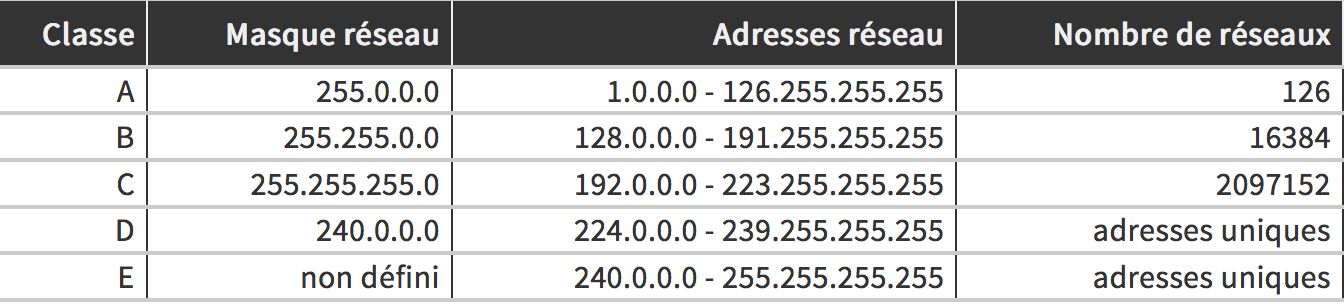
\includegraphics[scale=0.38]{masq.png}
	
	\textbf{Le routage} : Le routeur est un matériel de couche 3 qui relie plusieurs réseaux.
	\begin{itemize}
		\item Quand le routeur reçoit la trame, il vérifie qu'adresse MAC est bien la bonne, et ensuite il utilise la table de routage qui va donc lister les routeurs auxquels je peux envoyer mon datagramme pour joindre une destination donnée.
		\item La table de routage contient : la liste des réseaux que l'on peut joindre et les passerelles par lesquelles je dois passer pour les joindre. Construire une table de routage se fait en 3 étapes :
		\item indiquer les réseaux auxquels ma machine est connectée ;
		\item indiquer la route par défaut ;
		\item indiquer tous les autres réseaux que je ne peux pas encore joindre avec les deux étapes précédentes.
	\end{itemize}

	\textbf{Le protocole ARP :} On veut connaître le chemin pour envoyer un message à une machine, sauf que l'on a pas son adresse MAC, il existe un protocole pour remédier à cela : ARP.
	\begin{itemize}
		\item On envoie un message de \emph{broadcast}, en demandant à la personne dont on connait l'adresse IP de nous envoyer son adresse MAC : c'est la requête ARP.
		\item Sauf que si on envoie une requête à chaque fois que l'on veut transmettre un message on risque de saturer le réseau, d'où la \textbf{table ARP}.
		\item la table ARP garde en mémoire provisoirement les relation \texttt{adresse MAC $\longleftrightarrow$ adresse IP}, la table est dynamique, elle la garde en mémoire environ 2 minutes.
		\end{itemize}
		\textbf{Le serveur DHCP} : On se rend donc bien compte qu'il serait bien d'avoir un mécanisme rapide et fiable pour adresser les machines d'un réseau. C'est là qu'entre en jeu le protocole DHCP.
		\begin{itemize}
		\item La première fonction d'un serveur DHCP est de fournir des adresses IP  aux machines en faisant la demande.
		\item Demande en \emph{broadcast} en passant par l'adresse MAC : \texttt{ff:ff:ff:ff:ff:ff}
			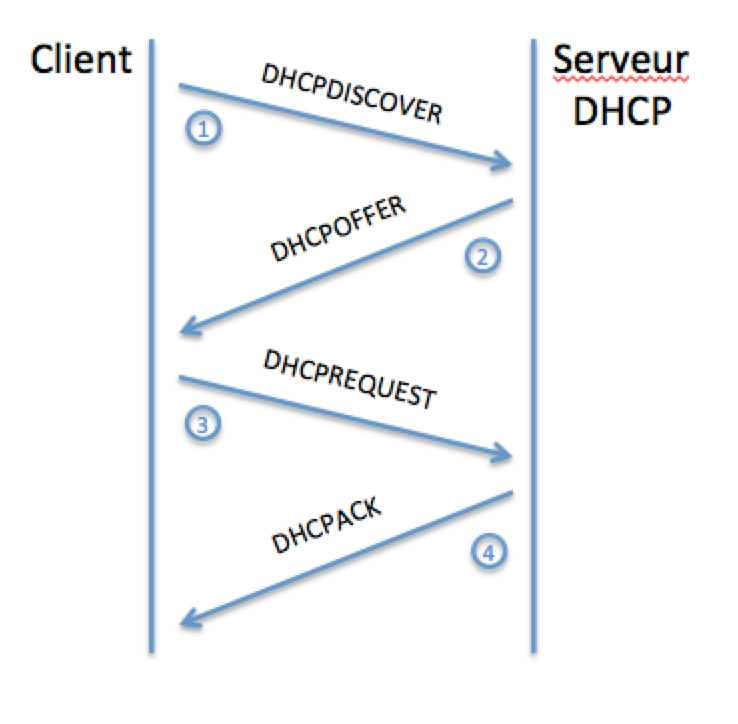
\includegraphics[scale=0.4]{dhcp.png}
	\end{itemize}
	
	\textbf{ICMP} : ICMP est un protocole dans la suite protocolaire TCP-IP utilisé pour envoyer des messages d'erreurs dans un réseau.
	Il travaille en partenariat avec le protocole IP.
	Nous allons le voir en détail, voir les différents types d'erreurs, leurs codes, leurs significations et les scénarios dans lesquels elles se manifestent.


\section*{Couche de transport}

	Deux principaux protocoles de transport : \textbf{TCP} et \textbf{UDP}.
	UDP : User Datagram Protocol .
	\begin{itemize}
		\item Très simple, aucune garantie que les messages arrivent ou arrivent dans l'ordre, mais les performances sont élevé (utilisé par exemple pour skype, le streaming,...).
		\item Utilisé beaucoup en téléphone IP et en DHCP.
	\end{itemize}
	
	TCP : Transmission Control Protocol.
	\begin{itemize}
		\item En 3 étapes : établissement de la connexion, transfert de données et fin de la connexion.
		\item Pendant la phase d'établissement de la connexion, des paramètres comme le numéro de séquence sont initialisés afin d'assurer une transmission fiable (sans perte et dans l'ordre) des données.
		\item Structure du segment TCP.
		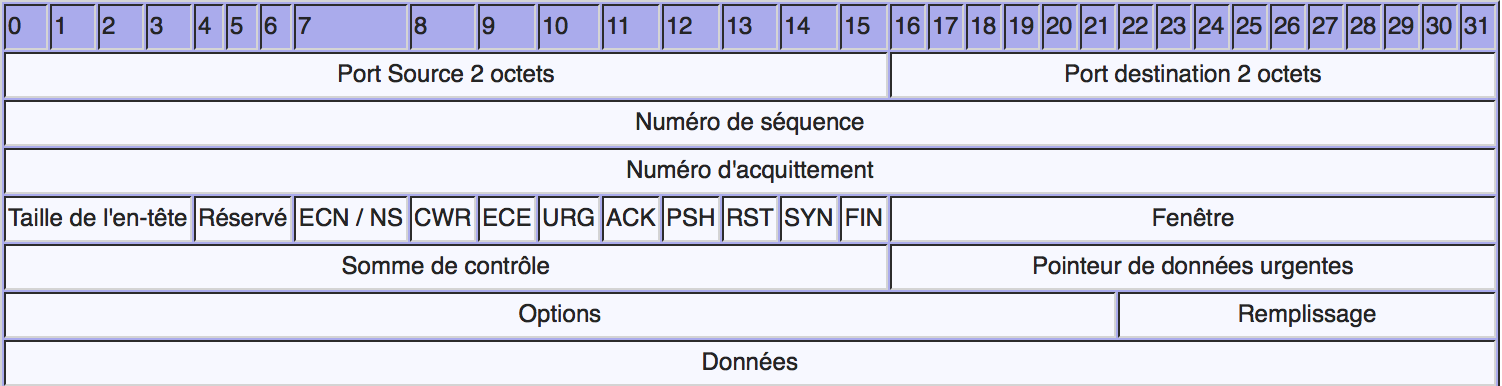
\includegraphics[scale=0.28]{tc.png}
		\item \textbf{Établissement d'une connexion :} un système ouvre une \emph{socket} et attend une demande de connexion d'un autre système, après c'est le \emph{three-way handshake}.
			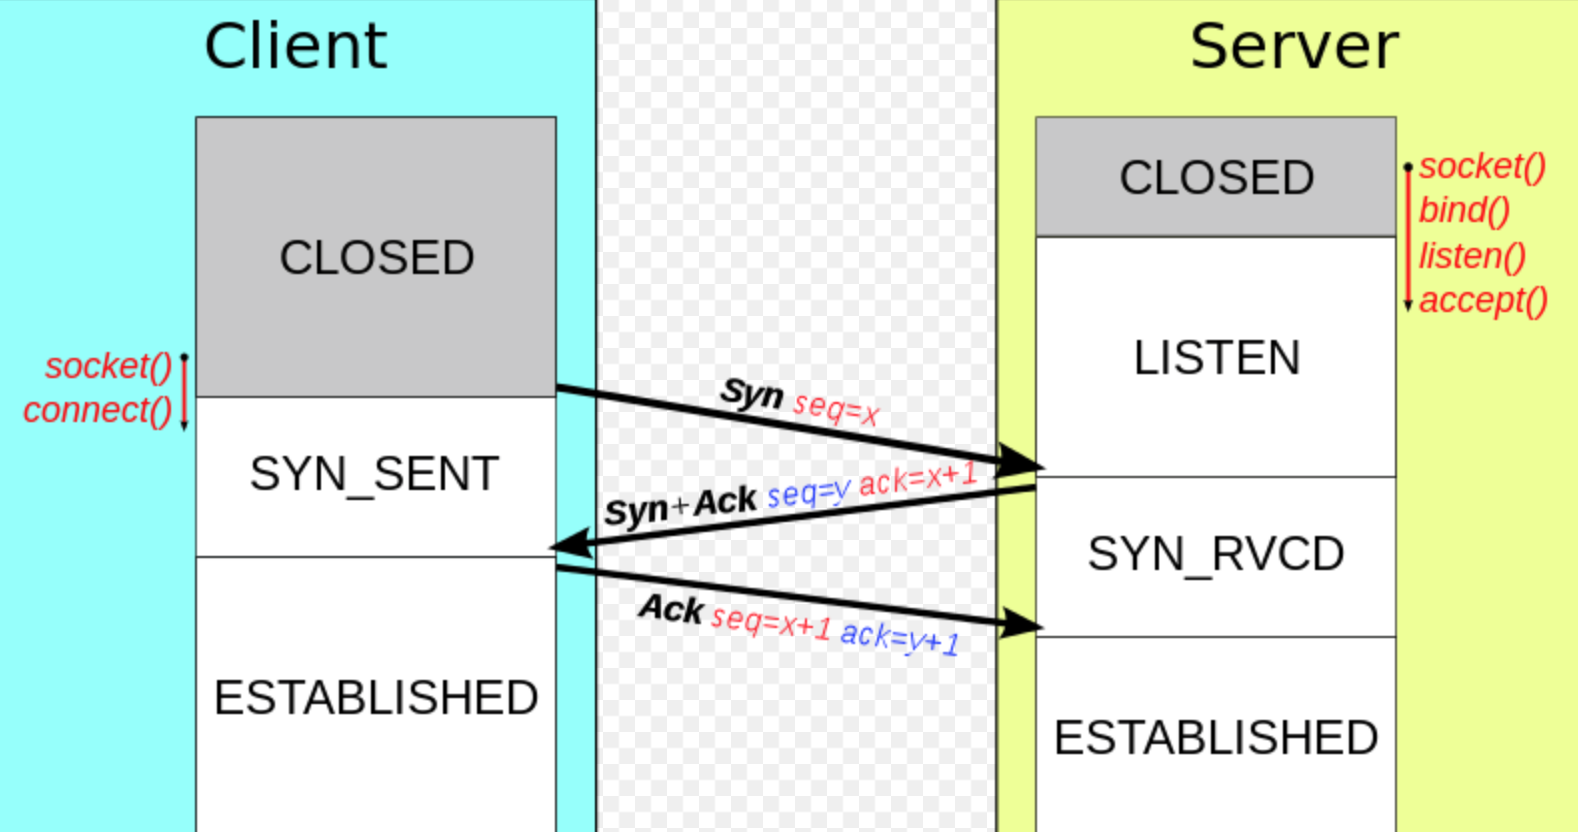
\includegraphics[scale=0.27]{hand.png}
		\item \textbf{Transfert de données :}
			certains mécanismes cléss permettent d'assurer la robustesse et la fiabilité de TCP.
			En particulier, les numéros de séquence sont utilisés afin d'ordonner les segments TCP reçus et de détecter les données perdues, les sommes de contrôle permettent la détection d'erreurs, et les acquittements ainsi que les temporisations permettent la détection des segments perdus ou retardés.
			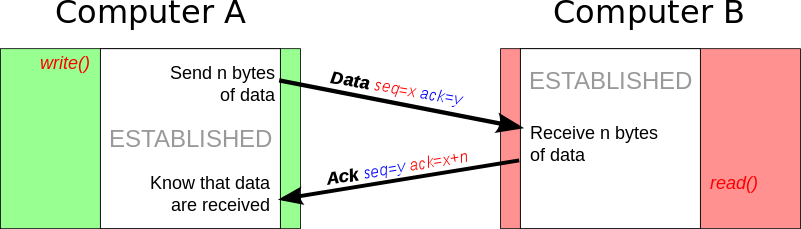
\includegraphics[scale=0.28]{trans.png}
		\item \textbf{Terminaison d'une connexion :}
			la phase de terminaison d'une connexion utilise un \emph{handshaking} en quatre temps, chaque extrémité de la connexion effectuant sa terminaison de manière indépendante.
			Ainsi, la fin d'une connexion nécessite une paire de segments FIN et ACK pour chaque extrémité.
			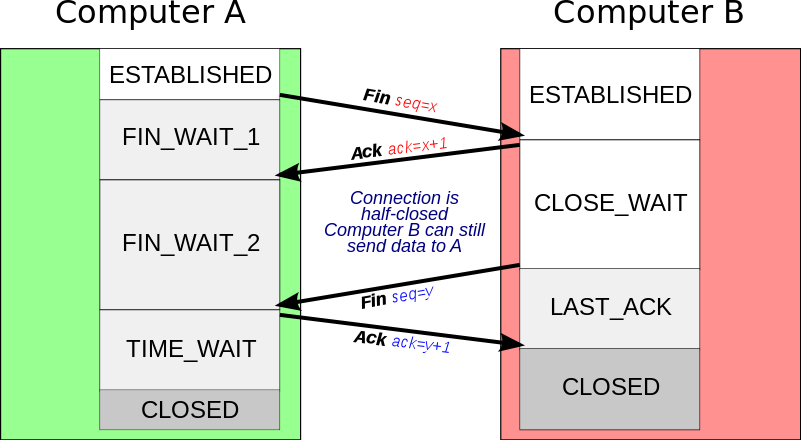
\includegraphics[scale=0.28]{term.png}
		\item \textbf{Contrôle de flux :}
			chaque partenaire dans une connexion TCP dispose d'un tampon de réception dont la taille n'est pas illimitée.
			Afin d'éviter qu'un hôte ne surcharge l'autre, TCP prévoit plusieurs mécanismes de contrôle de flux.
			Ainsi, chaque segment TCP contient la taille disponible dans le tampon de réception de l'hôte qui l'a envoyé.
			En réponse, l'hôte distant va limiter la taille de la fenêtre d'envoi afin de ne pas le surcharger.
		\item \textbf{Contrôle de congestion :}
			la congestion intervient lorsque trop de sources tentent d'envoyer trop de données trop vite pour que le réseau soit capable de les transmettre. Ceci entraîne la perte de nombreux paquets et de longs délais. Les émetteurs et destinataires TCP peuvent modifier le comportement du flux de données.
	\end{itemize}


\section*{Le service DNS}

	Domain Name System $\leftarrow$ indispensable au fonctionnement d'internet.
	Un nom de domaine se décompose en plusieurs parties.
	\begin{itemize}
		\item l'extension en premier : on parle de Top Level Domain.
			Il existe des TLD nationaux (fr, it, de, es, etc.) et les TLD génériques (com, org, net, biz, etc...).
			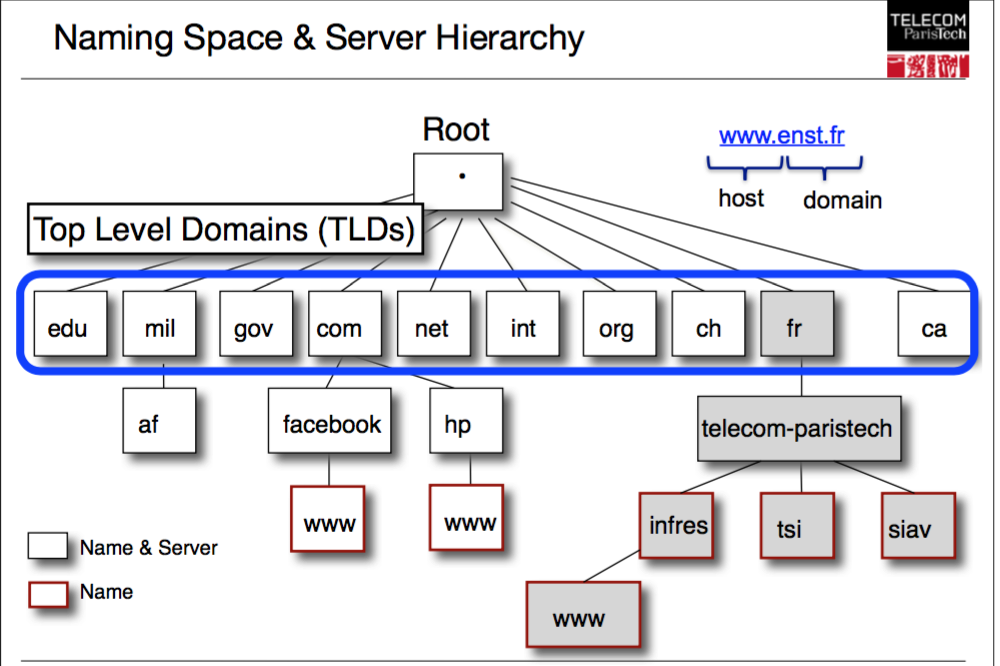
\includegraphics[scale=0.45]{dns.png}
		\item Le système de noms de domaine est géré par un organisme américain appelé l'ICANN.
			L'ICANN est responsable de la gestion des 13 serveurs DNS qui gèrent la racine du DNS.
			Ces 13 serveurs connaissent les adresses IP des serveurs DNS gérant les TLD (les .fr, .com, org, etc...).
	\end{itemize}

\end{document}